\documentclass[11pt]{article}
% Lightsmith technical report (arXiv). Build notes: paper/README.md; arXiv metadata: paper/ARXIV.md.
% The Python package is still imported as `lightsmith` while the rename to `lightsmith` lands.
\usepackage[T1]{fontenc}
\usepackage[utf8]{inputenc}
\usepackage{lmodern}
\usepackage[a4paper,margin=2.5cm]{geometry}
\usepackage{amsmath,amssymb}
\usepackage{graphicx}
\usepackage{booktabs}
\usepackage{tabularx}
\usepackage{xcolor}
\usepackage{listings}
\usepackage[numbers,sort&compress]{natbib}
\usepackage{url}
\usepackage[colorlinks=true,linkcolor=blue!50!black,citecolor=blue!50!black,urlcolor=blue!50!black]{hyperref}

\newcommand{\todo}[1]{\textcolor{red}{[TODO: #1]}}
\newcommand{\code}[1]{\texttt{#1}}
\newcommand{\npd}{n_\mathrm{pd}}
\newcommand{\Qabs}{Q_\mathrm{abs}}
\newcommand{\LS}{Lightsmith}
\graphicspath{{figures/}}

\lstset{basicstyle=\ttfamily\footnotesize,columns=fullflexible,breaklines=true,frame=single,
        showstringspaces=false}

\title{\LS: an open, GPU-native, differentiable photonics suite for humans and AI agents}
\author{Alexander Feghali\\ \small \todo{affiliation}}
\date{\todo{date}}

\begin{document}
\maketitle

% Keep in sync with the plain-text abstract in ARXIV.md.
\begin{abstract}
Photonics simulation is split between closed commercial suites and a fragmented landscape of
open single-method codes, each with its own input format, units, sign conventions and licence.
This makes cross-checking methods laborious for people and error-prone for the AI agents that are
increasingly asked to set up simulations. We present \LS{}, an MIT-licensed Python suite in which a
problem is described once, as a typed and JSON-serialisable specification covering seven problem
kinds (particle scattering, planar layer stacks, periodic structures, waveguide modes, devices,
photonic bands and circuits), and solved by any applicable backend on CPU or GPU. Native solvers
are written once against the Python array API, so the same code runs on NumPy and on PyTorch with
CUDA, and several are differentiable end to end. The suite includes Mie theory for multilayer
spheres, quasistatic models, a T-matrix interface, an FFT-accelerated discrete dipole approximation,
FDTD, transfer-matrix and rigorous coupled-wave analysis, mode solvers, frequency-domain inverse
design, plane-wave band structures and S-matrix circuits, with a CC0 database of measured optical
constants and passive Drude--Lorentz fitting. Every result carries provenance, and every
operation is exposed through a Python API, a JSON command-line interface and a Model Context
Protocol server, with a cheap estimate step before every expensive solve. We report validation of
each solver against analytic or independent references and a scripted cross-method benchmark of
scattering by dielectric and plasmonic particles, which quantifies how slowly and irregularly
volume-discretisation methods converge for metals. \todo{headline numbers from the full benchmark
and performance study.}
\end{abstract}

% ---------------------------------------------------------------------------
\section{Introduction}
\label{sec:intro}

\paragraph{Closed suites.} Industrial photonics design runs largely on commercial packages
that bundle FDTD, mode solvers, RCWA and circuit simulation behind one interface \todo{name
examples neutrally; no citation needed}. They are capable and well supported, but their solvers
are closed, their licences restrict redistribution and automation, and several now run only in a
vendor cloud.

\paragraph{Fragmented open tools.} The open-source alternatives are excellent but separate.
For particle scattering alone there are Mie codes \cite{Prahl2023miepython,PoinsinetdeSivry2023pymiesim,PenaPal2009},
T-matrix codes \cite{Beutel2024treams,Egel2021smuthi,Somerville2016smarties}, DDA codes
\cite{Draine1994,Yurkin2011adda,Wiecha2018pygdm,Ponomareva2025torchgdm} and FDTD codes
\cite{Oskooi2010meep,Mahlau2026fdtdx}, each with its own problem description, units,
time-harmonic sign convention, normalisation and licence (several are GPL). Comparing two methods
on the same problem, a basic sanity check, means writing two inputs and reconciling two sets of
conventions. Published cross-method comparisons are therefore mostly one-off studies
\cite{Parsons2010,Loke2014,Dieperink2024}, and even codes of one family agree to many digits only
when hidden parameters are aligned \cite{Argentin2026ddabench}. Each method also fails in its own
way: DDA and FDTD converge slowly for metals \cite{Yurkin2010gold,CalaLesina2015}, and RCWA needs
correct Fourier factorisation \cite{Li1996}.

\paragraph{Agents.} Large-language-model agents now design metasurfaces, multilayers, meta-optics
and photonic circuits
\cite{Lupoiu2025metachat,Kim2025llmphotonics,Huang2025mcp,Sharma2025phido,Wu2025picbench,Picopilot2026}.
Studies of such agents report that small, typed interfaces and fixed workflows are more reliable than
free-form scripting \cite{Huang2025mcp,Halo2026}, and that code which runs is often not correct
\cite{Mudur2025feabench}. Scattering and photonics codes rarely expose machine-readable schemas,
structured errors, pre-flight cost estimates or built-in cross-checks.

\paragraph{Contributions.} \LS{} provides:
\begin{enumerate}
  \item one typed problem specification for seven problem kinds, with fixed units and
  conventions, served identically through a Python API, a JSON CLI and an MCP server
  \cite{MCP2025spec}, with \code{estimate} before \code{solve} (Section~\ref{sec:arch});
  \item permissively licensed native solvers written against the Python array API standard
  \cite{ArrayAPI}, running on NumPy \cite{Harris2020numpy} and PyTorch \cite{Paszke2019pytorch}
  on CPU and CUDA GPUs, several differentiable (Section~\ref{sec:solvers});
  \item a bundled CC0 materials database with passive Drude--Lorentz fitting
  (Section~\ref{sec:materials});
  \item per-solver validation against analytic or independent references
  (Section~\ref{sec:validation}) and a scripted cross-method scattering benchmark with Mie theory
  as ground truth (Section~\ref{sec:bench});
  \item a CPU/GPU performance study (Section~\ref{sec:perf}).
\end{enumerate}

% ---------------------------------------------------------------------------
\section{Related work}
\label{sec:related}

\paragraph{Scattering codes.}
For spheres, miepython \cite{Prahl2023miepython} and PyMieSim \cite{PoinsinetdeSivry2023pymiesim}
(both MIT) compute Mie cross sections; scattnlay \cite{PenaPal2009} handles multilayer spheres under
the GPL. treams \cite{Beutel2024treams} (MIT) provides T-matrices for clusters, lattices and
stratified media; smuthi \cite{Egel2021smuthi} adds particles near planar interfaces; SMARTIES
\cite{Somerville2016smarties} targets spheroids; and a community T-matrix exchange format has been
proposed \cite{Asadova2025tmatrixformat}. DDSCAT \cite{Draine1994,DraineFlatau2013guide} and ADDA
\cite{Yurkin2011adda} are the reference DDA codes (GPL); pyGDM \cite{Wiecha2018pygdm} and TorchGDM
\cite{Ponomareva2025torchgdm} implement the Green dyadic method with dense matrices (GPL), and CPDDA
\cite{Xu2025cpdda} shows a CuPy FFT-DDA. Meep \cite{Oskooi2010meep} (GPL) is the reference open FDTD
code, and FDTDX \cite{Mahlau2026fdtdx} (MIT, JAX) targets GPUs and inverse design.

\paragraph{Other photonics solvers.} \todo{open TMM, RCWA, mode-solver, FDFD/inverse-design, PWE
and circuit codes; e.g.\ MPB \cite{JohnsonJoannopoulos2001mpb}; add only verified references.}

\paragraph{Multi-method toolkits.}
HoloPy wraps Mie, multisphere T-matrix and ADDA for holography (GPL, last release 2021); TorchGDM
couples GDM with effective models from Mie and T-matrix solutions; commercial suites unify many
methods behind closed solvers. To our knowledge no open package dispatches one declarative
problem description to this range of methods with consistent units, conventions and outputs.
\todo{re-check before submission; the survey behind this section is docs/landscape.md.}

\paragraph{Cross-method benchmarks.}
Wriedt and Comberg compared DDA, volume-integral, FDTD and T-matrix codes on a dielectric cube
\cite{WriedtComberg1998}; Yurkin \emph{et al.}\ compared DDA and FDTD for dielectric spheres
\cite{Yurkin2007ddafdtd}; Myroshnychenko \emph{et al.}\ reviewed methods for gold nanoparticles
\cite{Myroshnychenko2008}; Hoffmann \emph{et al.}\ compared field solvers on plasmonic gap antennas
\cite{Hoffmann2009}; Parsons \emph{et al.}\ \cite{Parsons2010} and Loke \emph{et al.}\
\cite{Loke2014} compared several methods on gold spheres; Cal\`a Lesina \emph{et al.}\ quantified
FDTD mesh and precision requirements for noble metals \cite{CalaLesina2015}; Gallinet \emph{et
al.}\ reviewed standard problems in nanophotonics \cite{Gallinet2015}; Lalanne \emph{et al.}\
benchmarked quasinormal-mode solvers across groups \cite{Lalanne2019}; Dieperink \emph{et al.}\
compared DDA, FDTD, DGTD and BEM against Mie for a gold sphere and observed irregular DDA
convergence \cite{Dieperink2024}; and Argentin \emph{et al.}\ cross-verified three DDA codes
\cite{Argentin2026ddabench}. Yurkin \emph{et al.}\ showed that sub-10\% near-infrared absorption
errors for gold spheres require of the order of $10^7$ dipoles \cite{Yurkin2010gold}.

\paragraph{Agents for photonics simulation.}
Agents have designed metasurfaces with surrogate solvers \cite{Lupoiu2025metachat}, multilayers
\cite{Kim2025llmphotonics}, meta-optics through an MCP server around differentiable RCWA
\cite{Huang2025mcp}, and photonic integrated circuits \cite{Sharma2025phido,Wu2025picbench,Picopilot2026};
others close the loop with physical acceptance criteria \cite{Kharel2026,Biswas2026,Halo2026}.
FEABench \cite{Mudur2025feabench} evaluates agents on multiphysics modelling, and FermiLink
\cite{Fermilink2026} spans many simulation packages through an agent layer.
\todo{verify each specific claim against the full texts.}

% ---------------------------------------------------------------------------
\section{Architecture}
\label{sec:arch}

\subsection{Typed problem specification}
Every problem is a Pydantic \cite{Pydantic} model with a \code{kind} discriminator and a published
JSON Schema, so it can be validated, stored, diffed and generated by programs. Seven kinds exist
(Table~\ref{tab:kinds}). Listing~\ref{lst:spec} shows a complete scattering problem.

\begin{table}[t]
\centering\small
\begin{tabularx}{\linewidth}{@{}lXl@{}}
\toprule
Kind & Describes & Solvers \\
\midrule
\code{scattering} & particles (spheres, layered spheres, spheroids, cylinders) in a homogeneous host under plane-wave illumination; cross sections, near and far fields & Mie, quasistatic, T-matrix, DDA, FDTD \\
\code{layer\_stack} & planar multilayers, coherent and incoherent layers; $R$, $T$, $A$ & TMM, RCWA, FDTD \\
\code{periodic} & 1D/2D patterned layers on any lattice, conical incidence; diffraction efficiencies & RCWA, FDTD \\
\code{mode} & waveguide cross-sections, straight or bent; effective and group indices, loss, mode fields & FDE \\
\code{device} & 2D/3D structures (or GDS layouts) with ports; S-parameters & FDFD (2D), EME \\
\code{bands} & photonic crystals; band structures along $k$-paths & PWE \\
\code{circuit} & netlists of compact models; circuit S-matrices & circuit solver \\
\bottomrule
\end{tabularx}
\caption{Problem kinds (\code{src/lightsmith/problems.py}) and the backends that accept them. An
eighth kind, \code{optimization}, wraps a \code{device} problem with design regions and objectives
for inverse design (Section~\ref{sec:fdfd}).}
\label{tab:kinds}
\end{table}

\begin{lstlisting}[caption={A scattering problem: a 20\,nm-radius gold sphere in water. Solver options
are optional and keyed by method or backend.},label={lst:spec}]
{"particles": [{"shape": {"kind": "sphere", "radius_nm": 20},
                "material": {"kind": "library", "name": "Au", "dataset": "Johnson-Christy"}}],
 "medium_index": 1.33,
 "wavelengths": {"start_nm": 450, "stop_nm": 700, "num": 51},
 "options": {"dda": {"dipoles_per_diameter": 24}}}
\end{lstlisting}

\subsection{Conventions}
Lengths are in nanometres and wavelengths are vacuum wavelengths. The time dependence is
$e^{-i\omega t}$, so absorbing materials have $\operatorname{Im}\varepsilon>0$; backends built on
$e^{+i\omega t}$ conjugate at their boundary. Scattering cross sections are in nm$^2$ and
efficiencies are normalised by $\pi r_\mathrm{eq}^2$, with $r_\mathrm{eq}$ the volume-equivalent
radius of all particles. Layer stacks are listed from the superstrate (incidence side) to the
substrate; waveguides propagate along $+z$. Conventions change only with the schema version.

\subsection{Backend registry, plugins and licensing}
A backend subclasses \code{Backend} and implements \code{supports(problem)}, which says whether it
can solve a problem and if not why, and \code{solve(problem, device)}, plus optionally
\code{available()} and \code{estimate(problem, device)}. With \code{method="auto"} the most
accurate applicable backend is chosen (for scattering: Mie, then T-matrix, then DDA, then FDTD),
and the reasons others were skipped are returned. Third-party backends register through the
\code{lightsmith.backends} entry-point group. The core is MIT-licensed and depends only on
permissive packages; GPL solvers (e.g.\ a scattnlay \cite{PenaPal2009} wrapper) live in separate
plugin packages, so installing the core never changes the licence of a user's work.

\subsection{CPU and GPU through the array API}
Native solvers are written against the Python array API standard \cite{ArrayAPI} and receive a
device object that supplies the array namespace. One code path therefore runs on NumPy (CPU), on
PyTorch (CPU or CUDA) and, where useful, on CuPy. Precision is an option and is recorded in every
result's provenance. By default DDA and FDTD run in single precision on GPUs and double precision on
CPUs; TMM, RCWA and the circuit solver use double precision everywhere; PWE uses double precision
except for its dense solver on a GPU.

\subsection{Differentiability}
With PyTorch arrays, native solvers that avoid non-differentiable steps support automatic
differentiation: the native Mie solver is differentiable end to end; TMM, RCWA, FDFD and the circuit
solver declare themselves differentiable to the inverse-design module; and PWE exposes a
differentiable band-structure function. Gradients are checked against finite differences in the
test suite (Section~\ref{sec:validation}). FDFD gradients with respect to every
permittivity pixel come from one adjoint solve reusing the forward factorisation
\cite{Hughes2018adjoint}, and the inverse-design module performs density-based topology
optimisation \cite{BendsoeSigmund2004,Molesky2018} on any backend that implements a small
differentiable-backend protocol.

\subsection{Agent interfaces}
The CLI (\code{doctor}, \code{backends}, \code{schema}, \code{estimate}, \code{solve},
\code{compare}) reads and writes JSON; failures print \code{\{"error", "message"\}} to standard error
and exit with status 1. The MCP server exposes the same operations as tools. Error messages name the
offending field and suggest a fix (e.g.\ ``Mie handles spheres only, got `spheroid'; use `dda' or
`tmatrix'{}''). \code{estimate} never solves: for DDA it reports dipole count, grid, precision and
memory; for FDTD the grid, time step and expected number of steps. \code{compare} solves with several
methods and reports their differences, with Mie as the reference where it applies. Results carry
provenance (versions, device, precision, grid, iterations, residuals, run time) and warnings.
\todo{llms.txt and AGENTS.md; planned agent evaluation protocol, if kept in this report.}

% ---------------------------------------------------------------------------
\section{Solvers}
\label{sec:solvers}

\subsection{Mie theory}
Lorenz--Mie theory gives the exact solution for spheres \cite{Mie1908,BohrenHuffman1998}. miepython \cite{Prahl2023miepython} solves homogeneous spheres. The native solver handles
homogeneous and multilayer spheres, vectorised over wavelengths, with log-derivative downward
recursion \cite{Wiscombe1980}, Yang's upward recursions for the ratios $\psi_n/\xi_n$
\cite{Yang2003}, and layer-to-layer recursion of effective log derivatives
\cite{Yang2003,PenaPal2009}, so no Riccati--Bessel function is formed and nothing overflows even in
single precision. Truncation follows Wiscombe \cite{Wiscombe1980} for homogeneous and Pe\~na and Pal
\cite{PenaPal2009} for layered spheres. It also returns near fields (by matching tangential fields
at each interface) and far fields, and is differentiable with respect to radii and permittivities.

\subsection{Quasistatic models}
For particles much smaller than the wavelength: Rayleigh spheres, coated spheres and Gans spheroids
\cite{BohrenHuffman1998}, optionally with radiative damping, the modified long-wavelength
approximation \cite{MeierWokaun1983,Kelly2003}, or a sphere polarisability from the Mie dipole
coefficient expanded to fourth order in the size parameter.

\subsection{T-matrix}
The T-matrix (null-field) method \cite{Waterman1965} is available for spheres, layered spheres and their clusters through treams \cite{Beutel2024treams}: each particle
gets its Mie T-matrix, clusters are coupled by solving the multiple-scattering problem, and
orientation averages use analytic trace formulas \cite{Mishchenko1991}. The wrapper performs
translations along $z$ combined with rotations, and solves a $\sqrt{|T|}$-scaled system, which its
author reports to be about 7 times faster than treams' own cluster path and stable for closely spaced
gold dimers. The multipole order follows Wiscombe's rule plus extra orders calibrated on the gap, with
an automatic convergence check. treams was not installed when the smoke benchmark ran
(Section~\ref{sec:bench}).

\subsection{Discrete dipole approximation}
\label{sec:dda}
The particle is replaced by point dipoles on a cubic lattice \cite{Purcell1973,Draine1994,Yurkin2007review}. The
dipole moments $\mathbf{P}_j$ solve
\begin{equation}
  \alpha_j^{-1}\mathbf{P}_j - \sum_{k\neq j}\mathsf{G}(\mathbf{r}_j-\mathbf{r}_k)\,\mathbf{P}_k
  = \mathbf{E}_\mathrm{inc}(\mathbf{r}_j),
\end{equation}
with $\mathsf{G}$ the free-space dipole tensor in the host and $\alpha_j$ the lattice-dispersion-relation
polarisability \cite{DraineGoodman1993}. The block-Toeplitz interaction is applied with FFTs on a
zero-padded grid in $O(N\log N)$ \cite{Goodman1991} and the system is solved with BiCGStab.
Cross sections follow Draine and Flatau \cite{Draine1994}:
\begin{equation}
  C_\mathrm{ext} = 4\pi k\sum_j \operatorname{Im}(\mathbf{E}_{\mathrm{inc},j}^{*}\cdot\mathbf{P}_j),\qquad
  C_\mathrm{abs} = 4\pi k\sum_j\Big[-\operatorname{Im}(\alpha_j^{-1})-\tfrac{2}{3}k^3\Big]|\mathbf{P}_j|^2 .
\end{equation}
Three discretisation modes are provided: \code{center} (default; sites whose centre lies inside,
with the lattice rescaled to the true volume), \code{weighted} (experimental; boundary sites mix
polarisabilities by supersampled volume fraction) and extrapolation (experimental; several
resolutions extrapolated to zero dipole size \cite{Yurkin2006extrap}). The resolution is set in
dipoles per diameter, $\npd$. Orientation averaging, near and far fields are supported. To our
knowledge this is the first permissively licensed FFT-accelerated DDA that runs on GPUs.
\todo{re-check this claim against docs/landscape.md before submission.}

\subsection{Finite-difference time domain}
A Yee grid \cite{Yee1966} with convolutional PML \cite{Roden2000cpml}, a total-field/scattered-field
plane-wave source, Drude--Lorentz dispersion through auxiliary differential equations as in Meep
\cite{Oskooi2010meep}, and anisotropic subpixel smoothing \cite{Farjadpour2006}, extended to dispersive
media. One broadband pulse covers all wavelengths; running DFTs of the fluxes through closed surfaces
give $C_\mathrm{sca}$ and $C_\mathrm{abs}$. On CUDA the time loop is replayed as CUDA graphs. Measured
materials are fitted with a passive Drude--Lorentz model first (Section~\ref{sec:materials}). The
same engine handles periodic structures and layer stacks at normal incidence, validated against TMM and
RCWA.

\subsection{Transfer-matrix method and RCWA}
The TMM solves planar multilayers with a stable recursion in which every phase factor decays, and
cascades thick incoherent layers in intensity \cite{KatsidisSiapkas2002}. RCWA (the Fourier modal
method) solves 1D and 2D periodic stacks, including non-rectangular lattices and conical incidence,
in a stable formulation \cite{Moharam1995} with correct Fourier factorisation \cite{Li1996} and its
2D normal-vector generalisation \cite{Schuster2007}. Fourier coefficients come from closed-form
transforms or supersampled rasters, layers are combined with Redheffer star products, and per-order
efficiencies are returned. Both solvers are vectorised over angle and wavelength, run on CPU and GPU, and
are differentiable with respect to thicknesses, permittivities and pixel maps.

\subsection{Mode solvers and eigenmode expansion}
The finite-difference eigenmode (FDE) solver computes full-vector modes of waveguide cross-sections on
a Yee grid with interface-aware permittivity averaging, PEC/PMC symmetry planes, PML, an exact
conformal transform for bends and shift-invert ARPACK. It returns effective and group indices
(including material dispersion), loss, mode fields and effective areas, and tracks modes across
wavelengths. The eigenmode expansion (EME) solver slices a device between two port planes into
piecewise-uniform cells (adaptively for tapers), takes each cell's modes from the FDE engine, and
cascades interface S-matrices from mode overlaps; cached modes make length sweeps cheap.

\subsection{FDFD and inverse design}
\label{sec:fdfd}
The FDFD solver treats 2D photonic devices with the scalar Helmholtz equation on a Yee grid with
stretched-coordinate PML, launches port modes computed on the same discretisation, and extracts
power-normalised, multimode S-matrices by modal decomposition. Linear solves are direct (SuperLU on
CPU; a block-tridiagonal LU in PyTorch on CUDA). Gradients come from one adjoint solve
\cite{Hughes2018adjoint}, which drives density-based topology optimisation with export of the
optimised layout to GDS \cite{BendsoeSigmund2004,Molesky2018}. The optimiser applies density
filtering, projection with continuation of the projection strength, minimum-feature penalties and
symmetry, with S-parameter and field objectives, MMA, Adam or L-BFGS-B, and checkpointing. The FDFD
solver is two-dimensional; 3D devices use EME.

\subsection{Plane-wave expansion}
Photonic band structures of lossless, non-dispersive 2D (TE and TM) and 3D crystals in a transverse
plane-wave basis, with the inverse-matrix Fourier rule of Ho, Chan and Soukoulis \cite{Ho1990} and
iterative eigensolvers in the spirit of MPB \cite{JohnsonJoannopoulos2001mpb}: a dense solver for TM
and a matrix-free LOBPCG solver with subpixel-smoothed permittivity for TE and 3D. It also computes band
gaps, densities of states and supercells for defect waveguides and cavities.

\subsection{Circuits and layout}
An S-matrix circuit solver interconnects compact models from netlists, on CPU or GPU and
differentiably, and reads Touchstone files. Layouts enter through a built-in GDSII reader, which
extrudes polygons into 3D structures, and through optional gdsfactory import of components and
netlists. The compact-model library covers waveguides, bends, couplers, MMIs, Y-branches, phase
shifters, ring and racetrack resonators, grating couplers and terminators, and any measured or
simulated S-matrix file.

% ---------------------------------------------------------------------------
\section{Materials}
\label{sec:materials}
\LS{} ships a pinned snapshot of measured optical constants from the refractiveindex.info database
\cite{Polyanskiy2024,refractiveindexinfo}, which is dedicated to the public domain (CC0). Each
material, e.g.\ \code{\{"kind": "library", "name": "Au", "dataset": "Johnson-Christy"\}}
\cite{JohnsonChristy1972}, carries its source paper, DOI and range of validity, and requests outside
that range fail with an explanatory error. The bundled set covers Au, Ag, Al and Cu (including
\cite{JohnsonChristy1972,Rakic1998,McPeak2015}), Si, SiO$_2$, TiO$_2$ and water; other entries can be
fetched from the database on demand.

Time-domain solvers need a rational permittivity. \code{fit\_drude\_lorentz} fits any material with a
Drude term plus Lorentz poles by bounded nonlinear least squares, with every parameter constrained so
that $\operatorname{Im}\varepsilon>0$ at all positive frequencies (passive, hence stable in FDTD). The
starting point comes from non-negative linear fits, continued pole by pole, so no user guess is
needed. The fit error is reported with the fit and in the provenance of every FDTD result.

% ---------------------------------------------------------------------------
\section{Validation}
\label{sec:validation}
Each solver is tested against an analytic solution, a high-precision reference or an independent
code. Every row cites its test file in \code{tests/}. Errors are labelled by provenance: \emph{bound}
is a tolerance the test asserts (an upper limit that every test run enforces); \emph{measured} is a
value recorded in the test file itself or in the smoke-benchmark output (\code{benchmarks/results/});
\emph{reported} is a value stated by the solver's author in the commit that added it or in their
report, not asserted by any test. \todo{Re-measure every ``reported'' entry with a script
in \code{benchmarks/} before submission, or drop it.}

\begin{table}[ht]
\centering\small
\begin{tabularx}{\linewidth}{@{}Xll@{}}
\toprule
Check & Reference & Error \\
\midrule
Homogeneous and coated spheres, hard cases & 40-digit mpmath & $10^{-11}$ bound; $\sim10^{-15}$ reported \\
Homogeneous spheres, Drude and dielectric & miepython & $<10^{-6}$ (bound) \\
Shell of core material vs.\ plain sphere & identity & $10^{-10}$ bound \\
$\int \mathrm{d}C_\mathrm{sca}/\mathrm{d}\Omega$ vs.\ $C_\mathrm{sca}$ & identity & $10^{-10}$ bound \\
GPU (double) vs.\ CPU & CPU & $10^{-12}$ bound; single precision $10^{-3}$ bound \\
Autograd gradient vs.\ finite differences & central differences & $10^{-6}$ bound \\
Smoke benchmark spheres (Section~\ref{sec:bench}) & miepython & $\le 6\times10^{-12}$ measured (5 spheres) \\
scattnlay plugin (GPL, separate package) & miepython & $10^{-9}$ bound; $10^{-11}$ reported \\
\bottomrule
\end{tabularx}
\caption{Native Mie solver (\code{tests/test\_mie\_native.py}).}
\label{tab:val-mie}
\end{table}

\begin{table}[ht]
\centering\small
\begin{tabularx}{\linewidth}{@{}Xll@{}}
\toprule
Check & Reference & Error \\
\midrule
5\,nm dielectric sphere, all corrections & Mie & $<1\%$ (bound) \\
5\,nm metal sphere, Mie-dipole correction & Mie & $<1\%$ (bound); ordering Mie-dipole $<$ MLWA $<$ none \\
Coated sphere & native Mie & $<1\%$ (bound) \\
Depolarisation factors, far-field integral & analytic & $10^{-12}$ bound \\
Smoke benchmark (larger particles, outside validity) & Mie & 15\% (Au, $r=20$\,nm) to 160\% (Ag, $r=30$\,nm) measured \\
\bottomrule
\end{tabularx}
\caption{Quasistatic models (\code{tests/test\_quasistatic.py}).}
\label{tab:val-qs}
\end{table}

\begin{table}[ht]
\centering\small
\begin{tabularx}{\linewidth}{@{}Xll@{}}
\toprule
Check & Reference & Error \\
\midrule
Dielectric sphere, $\npd=20$ & Mie & 0.07\% reported \\
Sphere $n=1.5+0.02i$ in water, $r=40$\,nm, $\npd=12$ & Mie & $<1\%$ (bound) \\
$\int \mathrm{d}C_\mathrm{sca}/\mathrm{d}\Omega$ vs.\ $C_\mathrm{sca}$; sphere orientation average & identity & $10^{-3}$ bound \\
GPU (single) vs.\ CPU (double) & CPU & $10^{-3}$ bound \\
Drude sphere $\Qabs$, $r=40$\,nm, 700\,nm, $\npd=8$--$32$ & Mie (0.107) & 0.25--1.69, i.e.\ 130--1480\% (Table~\ref{tab:staircase}) \\
GPU (single) vs.\ CPU (double), smoke suite & CPU & $\le10^{-5}$ measured \\
\bottomrule
\end{tabularx}
\caption{DDA (\code{tests/test\_core.py}, \code{tests/test\_dda.py}, smoke benchmark).}
\label{tab:val-dda}
\end{table}

\begin{table}[ht]
\centering\small
\begin{tabularx}{\linewidth}{@{}Xll@{}}
\toprule
Check & Reference & Error \\
\midrule
Au (Johnson--Christy), 450--900\,nm & tabulated data & $<2\%$ RMS, $<5\%$ max bound; 1.2\% RMS reported \\
Ag (Johnson--Christy), 450--900\,nm & tabulated data & $<2\%$ RMS, $<5\%$ max bound; 1.2\% RMS reported \\
Recovery of a known Drude--Lorentz model & exact model & $10^{-6}$ bound \\
Bundled datasets & manifest and spot values & exact \\
\bottomrule
\end{tabularx}
\caption{Materials and Drude--Lorentz fitting (\code{tests/test\_materials.py}).}
\label{tab:val-mat}
\end{table}

\begin{table}[ht]
\centering\small
\begin{tabularx}{\linewidth}{@{}Xll@{}}
\toprule
Check & Reference & Error \\
\midrule
Single sphere, off-origin, oblique incidence & miepython & $<10^{-6}$ bound; $\sim10^{-12}$ measured \\
Layered sphere whose shell is core material & plain sphere & $<10^{-6}$ bound \\
Cluster T-matrix and cross sections & treams' own cluster path & $10^{-10}$ (T-matrix), $10^{-9}$ (cross sections) bound \\
Gold--dielectric dimer, orientation average & Gauss--Legendre quadrature over incidences & $10^{-6}$ bound \\
$\int \mathrm{d}C_\mathrm{sca}/\mathrm{d}\Omega$ vs.\ $C_\mathrm{sca}$, clusters & identity & $10^{-6}$ bound \\
Gold dimer, gap $R/4$ & self-convergence & $<10^{-3}$ bound; bonding mode red-shifts $\ge20$\,nm \\
Distant pair ($10$ diameters) & $2\times$ single sphere & $C_\mathrm{ext},C_\mathrm{abs}$: 0.6\% measured, 1\% bound \\
Speed vs.\ treams' own path & --- & $\sim7\times$ reported \\
\bottomrule
\end{tabularx}
\caption{T-matrix via treams (\code{tests/test\_tmatrix\_treams.py}).}
\label{tab:val-tmatrix}
\end{table}

\begin{table}[ht]
\centering\small
\begin{tabularx}{\linewidth}{@{}Xll@{}}
\toprule
Check & Reference & Error \\
\midrule
Dielectric sphere ($n=1.5$, $r=60$\,nm), 2\,nm mesh, $C_\mathrm{ext}$ & Mie & 0.40\% measured; 0.6\% bound \\
Dielectric sphere, 6/4/3/2\,nm mesh & Mie & 1.1/0.8/0.6/0.4\% reported \\
Layered sphere, oblique incidence, 5\,nm mesh, $C_\mathrm{ext}$ & native Mie & $<3\%$ bound; 0.6\% (layered), $\sim$1\% (oblique) reported \\
Same, near-field enhancement (RMS) & native Mie & $<6\%$ bound \\
Drude sphere, plasmon peak, 2\,nm mesh & Mie & position $\le4$\,nm, height $<15\%$ bound \\
Drude sphere, plasmon peak, 1.33\,nm mesh & Mie & height $<7\%$ bound \\
Au (Johnson--Christy fit), $r=40$\,nm, 2\,nm mesh & Mie & position $\le10$\,nm, height $<20\%$ bound; peak at the Mie position, $-3.9\%$, 16\,s on an RTX~5070 reported \\
GPU (single) vs.\ CPU (double) & CPU & $10^{-4}$ bound; $\sim10^{-7}$ reported \\
Layer stacks: slab, Drude and Ag films & TMM & max $|\Delta R|,|\Delta T|$ 0.006, 0.0025, 0.004 measured \\
Lamellar grating; hole-array resonance & RCWA & 0.006 (0.012 at the Rayleigh anomaly); 0.09\,nm shift measured \\
\bottomrule
\end{tabularx}
\caption{FDTD (\code{tests/test\_fdtd.py}, \code{tests/test\_fdtd\_periodic.py}). The off-resonance
Drude absorption in the smoke benchmark is discussed in Section~\ref{sec:limits}.}
\label{tab:val-fdtd}
\end{table}

\begin{table}[ht]
\centering\small
\begin{tabularx}{\linewidth}{@{}Xll@{}}
\toprule
Check & Reference & Error \\
\midrule
Single interface, $r$ and $t$ amplitudes & Fresnel equations & $10^{-13}$ bound \\
$R_p$ at the Brewster angle & 0 & $<10^{-28}$ bound \\
Total internal reflection & $R=1$, $T=0$ & $10^{-14}$ bound \\
Quarter-wave AR coating; single film & 0; Airy formula & $<10^{-28}$; $10^{-14}$ bound \\
Bragg mirror, stop-band centre & analytic admittance & $10^{-12}$ bound \\
Thick incoherent slab & closed form & $10^{-10}$ bound \\
Unpatterned stack & TMM vs.\ RCWA & $10^{-12}$ bound \\
Lossless 1D conical and 2D hexagonal gratings & energy conservation & $10^{-12}$ bound \\
Rytov effective-medium limit (extrapolated) & analytic & $2\times10^{-5}$ (TE), $5\times10^{-5}$ (TM) bound \\
Metallic lamellar grating, TM, Li's rule & 80 harmonics & monotone; $<4\times10^{-3}$ at 40 harmonics bound; Laurent rule $>5\times$ worse \\
Gradients (thickness, permittivity, pixels) & finite differences & $10^{-6}$ (TMM), $10^{-4}$--$10^{-5}$ (RCWA) bound \\
GPU vs.\ CPU & CPU & $10^{-12}$ (TMM), $10^{-9}$ (RCWA) bound; GPU 2--8$\times$ faster reported \\
\bottomrule
\end{tabularx}
\caption{TMM and RCWA (\code{tests/test\_tmm.py}, \code{tests/test\_rcwa.py}).}
\label{tab:val-tmm}
\end{table}

\begin{table}[ht]
\centering\small
\begin{tabularx}{\linewidth}{@{}Xll@{}}
\toprule
Check & Reference & Error \\
\midrule
FDE: symmetric slab, TE and TM & dispersion relation & $<10^{-4}$ bound, second order; $\sim2\times10^{-6}$ reported \\
FDE: step-index fibre HE$_{11}$ & exact vector eigenvalue equation & $2\times10^{-6}$ bound; $5\times10^{-7}$ reported \\
FDE: Si strip $500\times220$\,nm, TE$_0$, 1550\,nm & SiPkit model, 2.44523 \cite{SiPkitNeff} & $3\times10^{-4}$ bound; 2.4453 reported \\
FDE: bend loss & exponential in radius & monotone (bound) \\
EME: uniform 3D guide & $|S_{21}|=1$, no reflection & $10^{-6}$; $10^{-8}$ bound \\
EME: width step & reciprocity & $10^{-6}$ bound \\
EME: linear taper, 1/3/10/30\,\textmu m & adiabatic limit & monotone, $<0.6$ and $>0.98$ at the ends (bound); 0.39/0.77/0.97/0.99 reported \\
EME: 1$\times$2 MMI \cite{SoldanoPennings1995} & symmetry; self-imaging length & 50/50 to $10^{-6}$ bound; best length within 10\% and transmission $>0.9$ (bound); 0.92 at $0.93\times$ reported \\
\bottomrule
\end{tabularx}
\caption{FDE mode solver and EME (\code{tests/test\_fde.py}, \code{tests/test\_eme.py}).}
\label{tab:val-fde}
\end{table}

\begin{table}[ht]
\centering\small
\begin{tabularx}{\linewidth}{@{}Xll@{}}
\toprule
Check & Reference & Error \\
\midrule
Straight guide, $|S_{21}|$ & 1 & $10^{-4}$ bound; $2\times10^{-9}$ reported \\
Closed guide with scatterers & power conservation; reciprocity & $10^{-6}$; $10^{-8}$ bound; $2\times10^{-8}$ (power) reported \\
Slab mode $n_\mathrm{eff}$ & analytic & $<10^{-3}$ bound, second order \\
Adjoint gradient & finite differences & $10^{-3}$ relative bound; $10^{-6}$ reported \\
GPU block-tridiagonal LU vs.\ CPU SuperLU & CPU & $10^{-10}$ bound; 2--5$\times$ faster on large grids reported \\
Inverse design: $2\times2$\,\textmu m Si bend & --- & objective rises monotonically, final $>0.8$, exported polygons within 0.15 (bound); $|S_{21}|^2=0.98$ with 100\,nm minimum features reported \\
\bottomrule
\end{tabularx}
\caption{FDFD and inverse design (\code{tests/test\_fdfd.py}, \code{tests/test\_inverse.py}).
\todo{Figures given by the module's author, $|S_{21}|^2=0.987$ (0.981--0.987 after export), $|S_{11}|^2\le2.5\times10^{-4}$
and reciprocity $8\times10^{-15}$ are not recorded in the repository; re-measure before use.}}
\label{tab:val-fdfd}
\end{table}

\begin{table}[ht]
\centering\small
\begin{tabularx}{\linewidth}{@{}Xll@{}}
\toprule
Check & Reference & Error \\
\midrule
Empty lattice, 2D and 3D fcc & free-photon bands & $10^{-6}$ bound \\
Square rods, $\varepsilon=8.9$, $r=0.2a$, TM gap & textbook value 31.4\% \todo{check against the book} & 0.3224--0.4425 (31.4\%) measured; 0.5\% bound on edges \\
Square rods, $\varepsilon=12$, TM gap & MPB tutorial, 0.282623--0.419335 \cite{MPBTutorial} & 0.28066--0.41717, i.e.\ within 0.7\% (measured); 1\% bound \\
Triangular air holes, $\varepsilon=13$, $r=0.48a$, complete gap & textbook value 18.6\% \todo{check against the book} & 0.4297--0.5199 (19.0\%) measured; 1\% bound on edges \\
Diamond lattice, $\varepsilon=11.56$ spheres, complete gap & --- & 0.2815--0.3144 (11.0\%) measured \\
Line-defect supercell & cf.\ \cite{Mekis1996} & one guided band in the gap (bound) \\
Differentiable bands & finite differences & $10^{-5}$ bound \\
GPU vs.\ CPU & CPU & $2\times10^{-4}$ (TM, single) and $10^{-6}$ (TE) bound; $\sim17\times$ faster in 3D reported \\
\bottomrule
\end{tabularx}
\caption{Plane-wave expansion (\code{tests/test\_pwe.py}).}
\label{tab:val-pwe}
\end{table}

\begin{table}[ht]
\centering\small
\begin{tabularx}{\linewidth}{@{}Xll@{}}
\toprule
Check & Reference & Error \\
\midrule
Mach--Zehnder interferometer & analytic bar/cross amplitudes & $10^{-12}$ bound \\
All-pass ring (netlist and model) & analytic formula & $10^{-10}$; $10^{-12}$ bound \\
Free spectral range & $\lambda^2/(n_g L)$ & 1\% bound \\
Critical coupling & zero transmission & $|S_{21}|^2<10^{-20}$ bound \\
Lossless circuits & unitarity; reciprocity & $10^{-12}$ bound \\
Gradients through a ring resonance & finite differences & $10^{-5}$ bound \\
GPU vs.\ CPU & CPU & $10^{-10}$ bound \\
\bottomrule
\end{tabularx}
\caption{Photonic circuits (\code{tests/test\_circuit.py}). \todo{The FSR comparison 9.080 vs.\
9.082\,nm is not recorded in the repository; re-measure before use.}}
\label{tab:val-circuit}
\end{table}

% ---------------------------------------------------------------------------
\section{Cross-method scattering benchmark}
\label{sec:bench}

\subsection{Protocol}
The benchmark is a set of scripts in \code{benchmarks/} (\code{problems.py}, \code{run.py},
\code{analyze.py}, \code{plots.py}). \code{problems.py} writes the problem suite as specifications;
\code{run.py} discovers the installed backends at run time and, for every problem, backend, device,
discretisation variant and resolution, records cross sections, the relative error against the
reference, wall time, peak memory (\code{tracemalloc} on CPU, \code{torch.cuda.max\_memory\_allocated}
on GPU), the pre-flight \code{estimate} and full provenance. Runs whose estimate exceeds a per-device
budget are skipped and logged. The reference is Mie theory whenever a Mie backend supports the
problem (homogeneous and layered spheres); otherwise the most accurate method present (T-matrix,
then DDA, then FDTD) at its highest resolution, labelled as such and reported with its
self-convergence. The headline error of a run is
\begin{equation}
  \epsilon = \max_{\lambda}\max\left(\frac{|C_\mathrm{ext}-C_\mathrm{ext}^\mathrm{ref}|}{C_\mathrm{ext}^\mathrm{ref}},
  \frac{|C_\mathrm{abs}-C_\mathrm{abs}^\mathrm{ref}|}{C_\mathrm{abs}^\mathrm{ref}}\right),
\end{equation}
omitting $C_\mathrm{abs}$ for (near-)lossless particles. For each resolution ladder we fit
$\epsilon\propto(\text{resolution})^{-p}$ and report the order $p$, the scatter of $\log_{10}\epsilon$
about the fit (``staircase noise'', in decades) and the fraction of refinements that reduce the
error. Following \cite{Argentin2026ddabench}, all solver parameters are recorded with every result.

\begin{table}[t]
\centering\small
\begin{tabularx}{\linewidth}{@{}lXl@{}}
\toprule
Family & Parameters (full suite) & Reference \\
\midrule
Dielectric spheres & $x\in\{0.5,1,2,5,10\}$, $m\in\{1.2,1.5,2,3.5\}$, lossless and lossy, vacuum and water & Mie \\
Au, Ag spheres & $r=10$--$100$\,nm, vacuum and water, Johnson--Christy data \cite{JohnsonChristy1972} & Mie \\
Drude sphere & $r=40$\,nm, water, 700\,nm; dense $\npd$ sweep & Mie \\
Core--shell & SiO$_2$@Au and Au@SiO$_2$, four sizes & Mie (layered) \\
Spheroids & Au, Ag; aspect ratio 1--5; $r_\mathrm{eq}=20$\,nm & highest resolution \\
Rods & Au, Ag flat-ended cylinders; aspect ratio 2--5 & highest resolution \\
Dimers & Au, Ag, $r=20$\,nm; gap 1--40\,nm & highest resolution \\
\bottomrule
\end{tabularx}
\caption{Benchmark problem families (145 problems in the full suite). The smoke suite uses one
problem per family with 1--3 wavelengths.}
\label{tab:suite}
\end{table}

\subsection{Smoke-suite results (preliminary)}
\label{sec:smoke}
\todo{Replace with full-suite results.} The numbers below come from the smoke suite
(Table~\ref{tab:suite}, one problem per family), run on an AMD Ryzen~5 5600X (NumPy, double precision) and an NVIDIA GeForce RTX~5070 (PyTorch 2.11, CUDA 12.8, single precision for DDA and FDTD), with the GPU shared with other jobs. The suite (98 runs, 127 planned runs skipped by budget or unsupported) took 649\,s; raw data are in \code{benchmarks/results/20261101-011025-smoke}. A first, longer run with every DDA variant on every problem (154 runs, 44\,min) is in \code{benchmarks/results/20261101-012216-smoke-extended}.

\paragraph{Exact methods.} The native Mie solver agrees with miepython to within
$6\times10^{-12}$ (maximum relative error of $C_\mathrm{ext}$ and $C_\mathrm{abs}$ over all sphere
problems), on CPU and GPU; it also provides the layered-sphere reference for the core--shell problem.

\paragraph{Dielectric sphere.} For a sphere with $n=1.995+0.01i$ in water (relative real index 1.5, size
parameter 1.5), centre-discretised DDA converges smoothly: the extinction error falls from 3.1\% at
$\npd=8$ to 0.87\% at $\npd=20$ (absorption: 4.8\% to 1.4\%), with fitted order $p=1.3$--$1.4$ and a
scatter about the power law of only 0.01 decades. FDTD with a 10.8\,nm mesh gives 2.5\% extinction
error (28\% for the weak absorption).

\paragraph{The staircase problem.} Table~\ref{tab:staircase} and Figure~\ref{fig:staircase} show the
Drude sphere. The DDA absorption efficiency does not converge monotonically: it jumps from 1.40 at
$\npd=10$ to 0.25 at 12, back up to 0.72 at 16, and settles near 0.275 for $\npd=24$--32, still 2.6
times the Mie value of 0.107 with 17\,000 dipoles. The power-law fit gives $p=1.5$ with 0.26 decades of
scatter (versus 0.01 for the dielectric sphere), and only 60\% of refinements reduce the error. The
experimental weighted discretisation does not help: in single precision on the GPU, BiCGStab reaches
the 3000-iteration cap for $\npd\ge12$ and broke down (NaN) at $\npd=24$. Extrapolation to zero dipole
size amplifies the noise ($\Qabs=6.9$, $-0.14$ and $1.15$ for ladders ending at $\npd=16$, 24 and 32).
FDTD converges monotonically but slowly ($\Qabs=1.20$, 0.82, 0.36 at 8, 4 and 2\,nm; order
$p\approx1$). \todo{The plateau at $\Qabs\approx0.275$ between $\npd=24$ and 32 suggests a systematic
error beyond staircase noise; investigate (polarisability prescription for $|m|\approx4$, absorption
formula) before the full run.}

\begin{table}[t]
\centering\small
\begin{tabular}{@{}lrrrrrrrrrrr@{}}
\toprule
$\npd$ & 8 & 10 & 12 & 14 & 16 & 18 & 20 & 22 & 24 & 28 & 32 \\
\midrule
DDA \code{center} & 1.69 & 1.40 & 0.25 & 0.41 & 0.72 & 0.32 & 0.46 & 0.31 & 0.28 & 0.28 & 0.27 \\
DDA \code{weighted} & 0.30 & & 0.54$^a$ & & 0.98$^a$ & & & & --$^b$ & & 0.35$^a$ \\
\bottomrule
\end{tabular}
\caption{$\Qabs$ of the Drude sphere versus dipoles per diameter (Mie: 0.107). $^a$BiCGStab stopped at
the 3000-iteration cap. $^b$Breakdown (NaN). CPU (double) and GPU (single) centre results agree to
$10^{-5}$ where both were run ($\npd=8,10$).}
\label{tab:staircase}
\end{table}

\paragraph{Gold, silver and core--shell spheres.} At the finest smoke resolutions, the extinction error
of DDA is 98\% for Au ($r=20$\,nm, $\npd=24$), 67\% for Ag ($r=30$\,nm in vacuum, $\npd=24$) and 48\% for
SiO$_2$@Au ($\npd=24$); absorption errors are larger. The smoke ladders are far too short for metals;
they test the pipeline, not convergence.

\paragraph{Non-spherical particles.} With only DDA available as a general method, the references for
the spheroid, rod and dimer are DDA solutions on the finest lattice, and they are not converged: the
change from the next coarser lattice is 47\%, 253\% and 30\% respectively. Errors quoted against these
references are therefore not meaningful yet; T-matrix references (treams) are needed.

\paragraph{Regime map.} With absorption included, no general-method run in the smoke suite reaches
10\% error on any metal problem (Figure~\ref{fig:regime}); for the dielectric sphere, DDA at $\npd=8$
on the CPU (0.15\,s) already meets 5\%.

\begin{figure}[t]
  \centering
  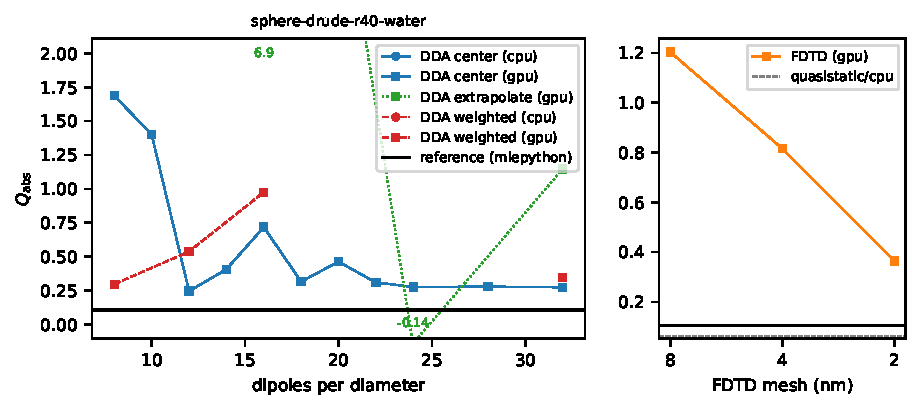
\includegraphics[width=\linewidth]{staircase_sphere-drude-r40-water.pdf}
  \caption{Absorption efficiency of a Drude sphere ($\varepsilon_\infty=9.5$, $\hbar\omega_p=9$\,eV,
  $\hbar\gamma=0.07$\,eV; $r=40$\,nm in water; $\lambda=700$\,nm) versus DDA resolution for the three
  discretisation modes on CPU and GPU (left) and versus FDTD mesh (right). Black: Mie theory.
  Smoke suite.}
  \label{fig:staircase}
\end{figure}

\begin{figure}[t]
  \centering
  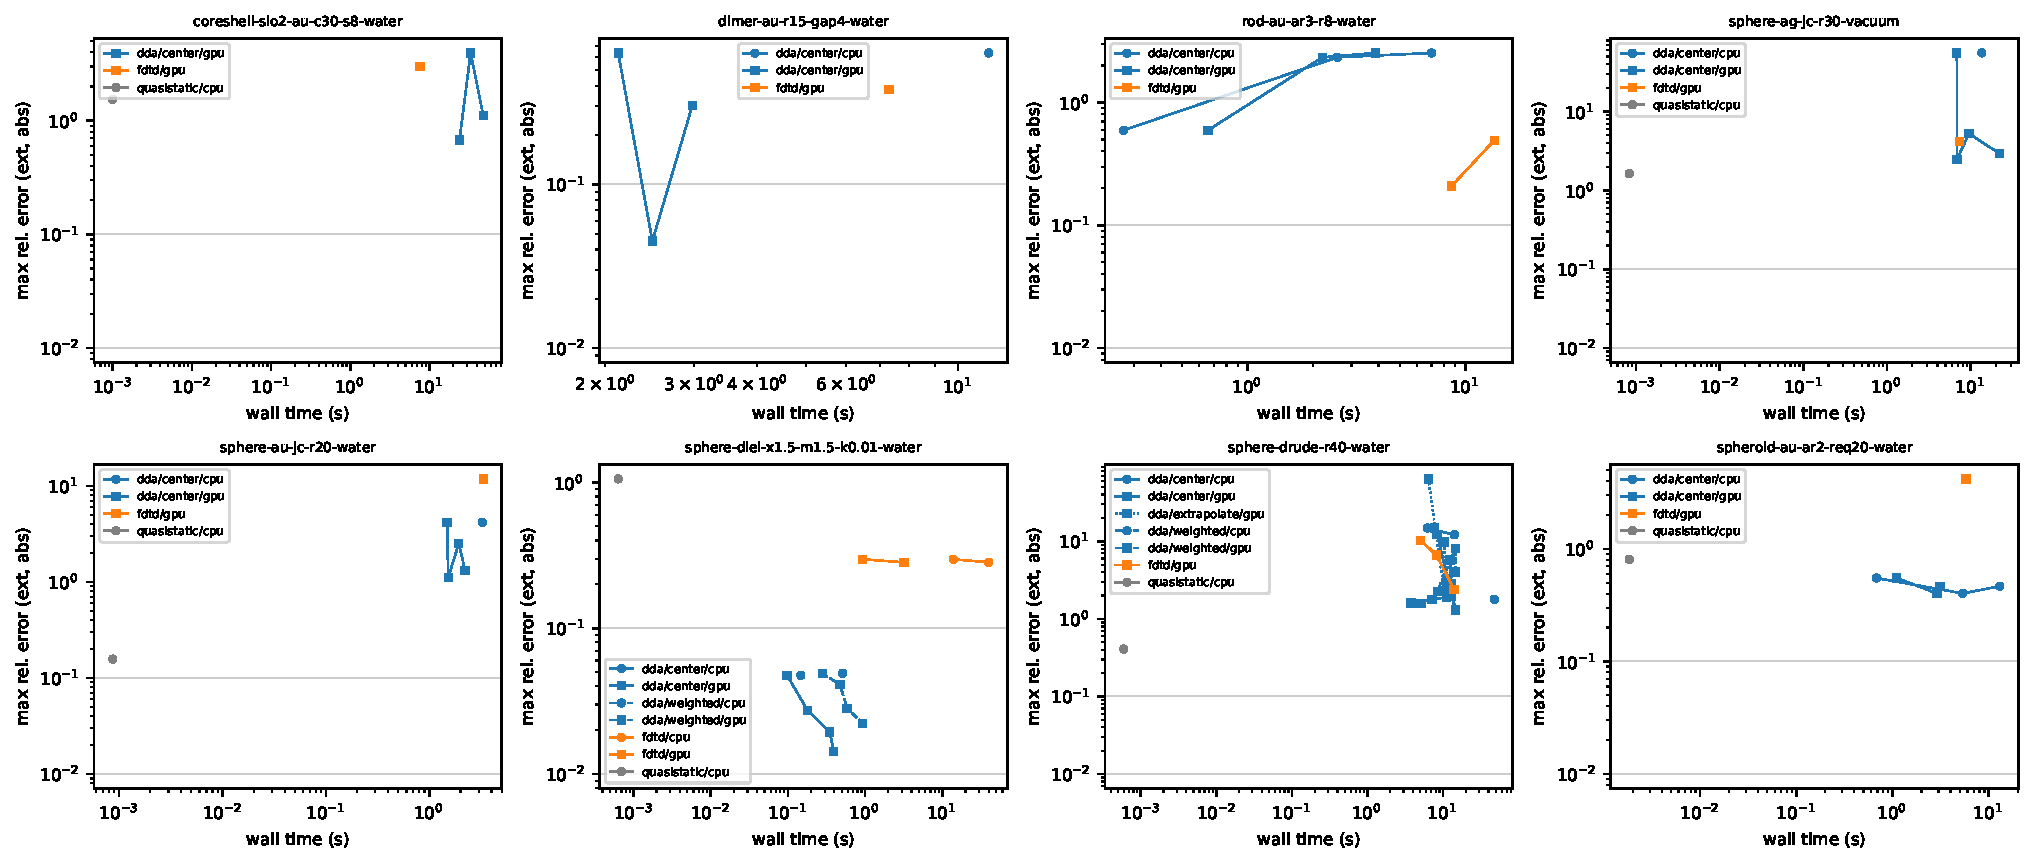
\includegraphics[width=\linewidth]{error_vs_cost.pdf}
  \caption{Headline error versus wall time for every run of the smoke suite; lines join the
  resolution ladder of one backend, variant and device.}
  \label{fig:cost}
\end{figure}

\begin{figure}[t]
  \centering
  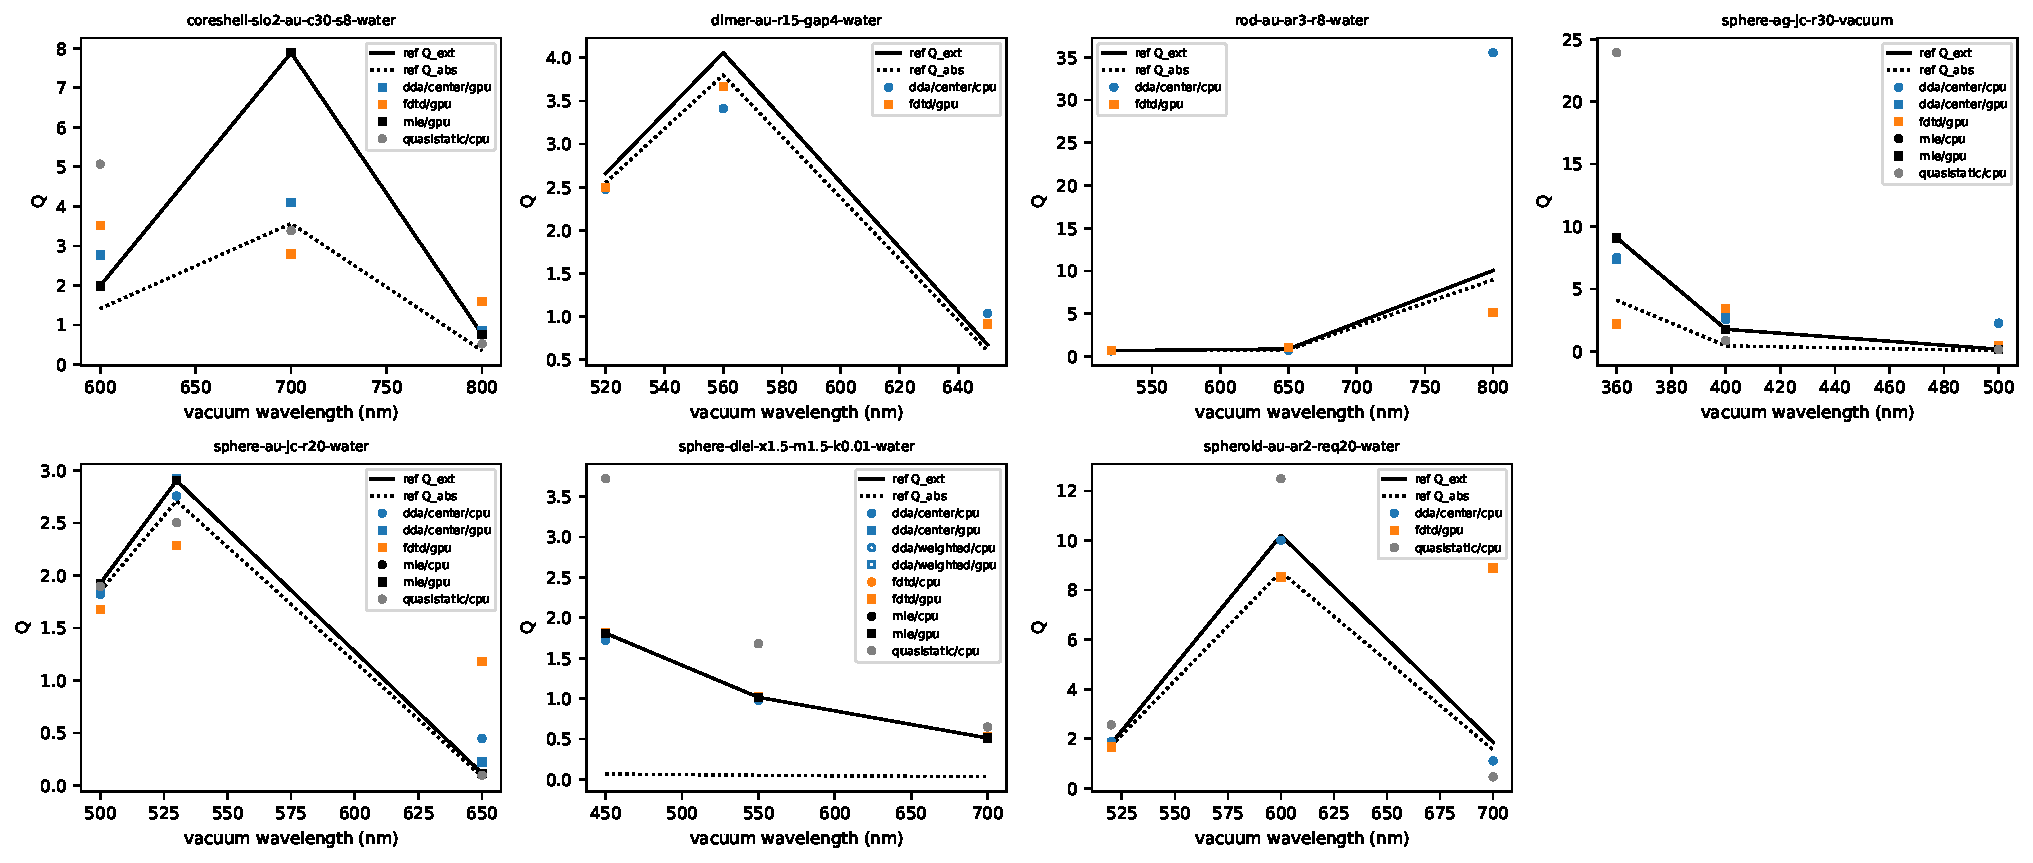
\includegraphics[width=\linewidth]{spectra.pdf}
  \caption{Extinction efficiency at the finest resolution of each backend (markers) against the
  reference (black). Smoke suite (three wavelengths per problem).}
  \label{fig:spectra}
\end{figure}

\begin{figure}[t]
  \centering
  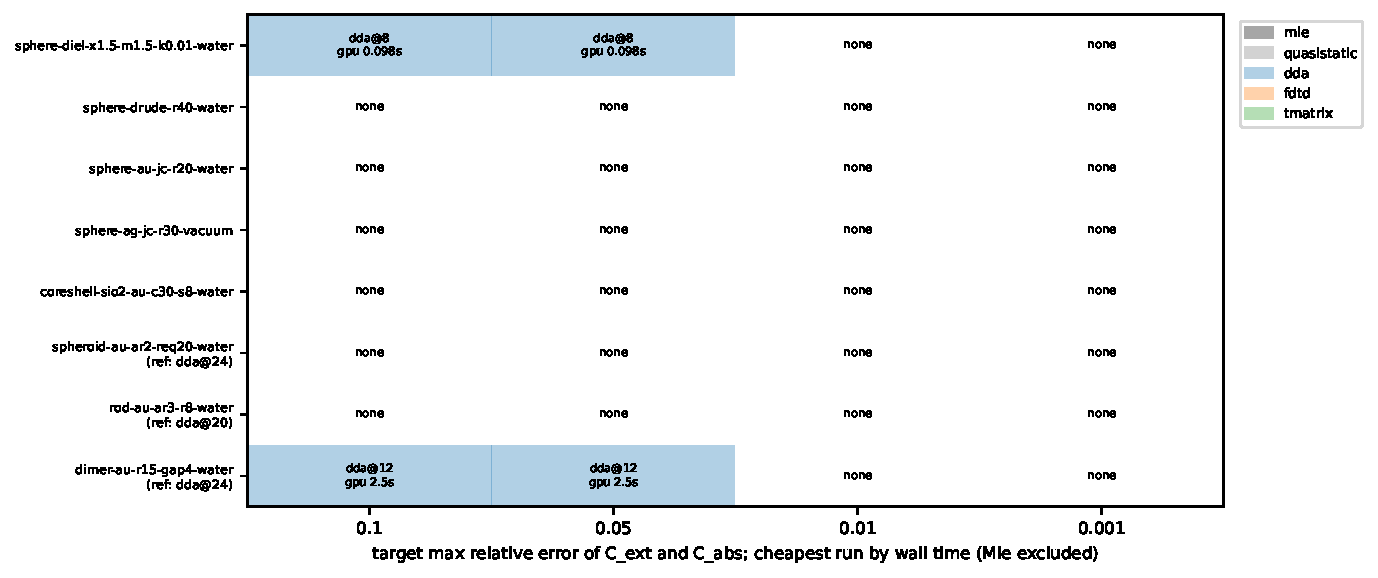
\includegraphics[width=0.85\linewidth]{regime_map.pdf}\[1ex]
  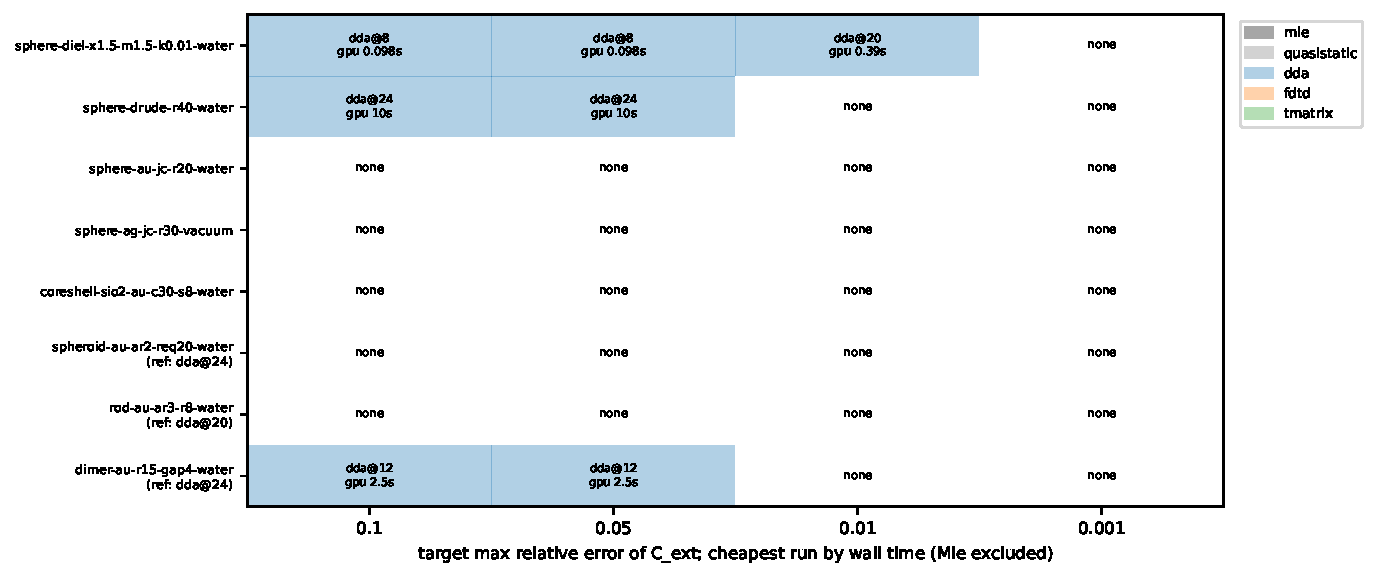
\includegraphics[width=0.85\linewidth]{regime_map_ext.pdf}
  \caption{Cheapest run (by wall time, Mie excluded) meeting each target accuracy, for the headline
  error (top) and for extinction only (bottom); ``none'': no run of the ladder reached it. Non-Mie
  references are labelled on the axis. Smoke suite.}
  \label{fig:regime}
\end{figure}

\subsection{Full suite}
\todo{Accuracy versus cost per family; regime maps on physical axes; DDA convergence order and
staircase noise for metals; weighted versus centre discretisation; value of extrapolation; GPU single
versus double precision; FDTD fit error; T-matrix versus DDA for dimers and spheroids.}

% ---------------------------------------------------------------------------
\section{Performance: CPU versus GPU}
\label{sec:perf}
In the smoke suite, GPU and CPU results agree to about $10^{-6}$ (relative $C_\mathrm{ext}$), as
expected for single versus double precision. FDTD on the GPU was 12.5--14.8 times faster than on the
CPU for the dielectric sphere ($1.7$--$2.7\times10^5$ cells). For DDA, the CPU budget limited matched
comparisons to small lattices ($\le560$ dipoles), where the GPU was 0.4--6.7 times faster
(Figure~\ref{fig:gpu}); larger lattices ran on the GPU only. Separately, the native Mie solver is about
15 times faster on the GPU than on the CPU for $10^6$ wavelengths. Peak GPU memory was within a factor
of two of \code{estimate}: the DDA estimate was conservative (41\,MiB estimated vs.\ 26\,MiB measured),
the FDTD estimate low (14 vs.\ 22\,MiB); on the CPU the FDTD estimate was 3.7 times below the
\code{tracemalloc} peak. \todo{fix the FDTD memory estimate or document what it covers.}

\begin{figure}[t]
  \centering
  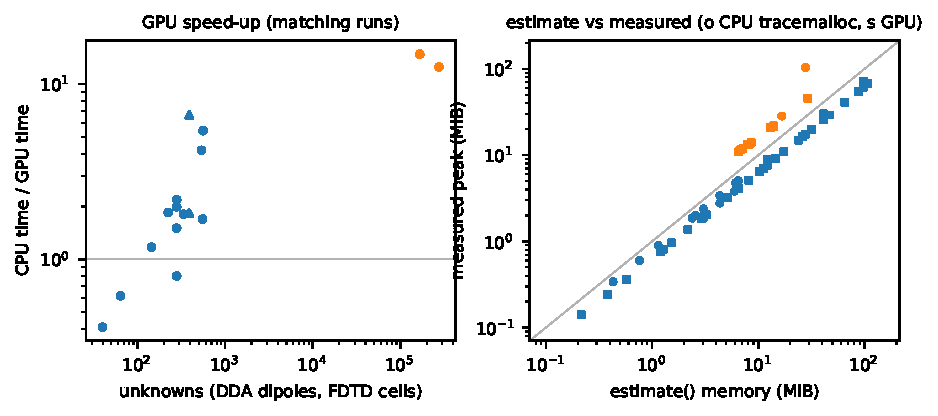
\includegraphics[width=\linewidth]{gpu_speedup.pdf}
  \caption{Left: CPU/GPU wall-time ratio for matching DDA and FDTD runs of the smoke suite. Right:
  memory predicted by \code{estimate} versus measured peak memory.}
  \label{fig:gpu}
\end{figure}

\todo{Systematic study on an idle machine: throughput versus problem size for every native solver,
single versus double precision, CPU thread count, energy.}

% ---------------------------------------------------------------------------
\section{Platform}
\label{sec:platform}
\todo{Short description of Studio, Cloud, Materials and Community, written by the platform authors
and limited to verifiable facts.}

% ---------------------------------------------------------------------------
\section{Limitations and roadmap}
\label{sec:limits}

\paragraph{Voxel methods and off-resonance metal absorption.} In the smoke benchmark, both
volume-discretisation methods overestimate the absorption of the Drude sphere ($r=40$\,nm in water,
$\lambda=700$\,nm, off resonance; Mie $\Qabs=0.107$) by a factor of 2.6--3.4 even at the finest
spacings we ran: DDA gives $\Qabs=0.274$ at $\npd=32$ (about 2.5\,nm dipole spacing; 2.6 times Mie),
with values between 0.274 and 0.278 from $\npd=24$ to 32, and FDTD gives $\Qabs=0.364$ on a 2\,nm mesh
(3.4 times Mie), still decreasing. Extinction is overestimated too, by 39\% (DDA) and 43\% (FDTD). The exact methods agree with each
other on the same problem: native Mie and miepython differ by $1.2\times10^{-12}$. We report this as a
measured observation and do not yet claim a mechanism. The FDTD test suite asserts much smaller errors
for the extinction peak at resonance ($<7\%$ on a 1.33\,nm mesh), so the discrepancy may be specific to
off-resonance absorption, where $\Qabs$ is small. It needs a dedicated study: finer meshes, double precision, other polarisability
prescriptions and an independent DDA code.

\begin{itemize}
  \item \textbf{References for non-spherical particles} in the benchmark are the highest-resolution
  solution of the best available method, not exact. For metals this is weak: the DDA absorption of a
  Drude sphere is still far from Mie at the finest lattice of the smoke suite. A T-matrix reference,
  cross-checked against converged FDTD, is needed for spheroids, rods and dimers.
  \item \textbf{Staircase error} dominates volume discretisations of metals and is non-monotonic in
  resolution \cite{Yurkin2010gold}; single-resolution DDA results for metals should be treated with
  caution, and extrapolation \cite{Yurkin2006extrap} does not remove the noise.
  \item \textbf{Iterative cost.} Unpreconditioned BiCGStab needs of the order of $10^3$ iterations for
  metals; better Krylov methods and preconditioners are planned.
  \item \textbf{Precision.} GPU runs default to single precision, and double precision is slow on
  consumer GPUs. \todo{quantify.}
  \item \textbf{Timing.} CPU memory is measured with \code{tracemalloc}, which slows Python-level loops;
  development runs shared the GPU with other jobs. \todo{final runs on an idle machine.}
  \item \textbf{Scope.} No substrates for particles, no non-local or quantum effects. \todo{roadmap:
  rename to \code{lightsmith}, 3D FDFD, substrates, further plugins.}
\end{itemize}

% ---------------------------------------------------------------------------
\section{Availability}
\label{sec:availability}
\LS{} is released under the MIT licence at \todo{repository URL} \todo{PyPI}. The benchmark
scripts, the problem suites (JSON) and the raw results of every run reported here (CSV and JSON with
provenance) are in \code{benchmarks/}. \todo{archive the release and results with a DOI at
submission.} Bundled optical constants come from the refractiveindex.info database (CC0)
\cite{Polyanskiy2024}; please also cite the original dataset papers listed with each material and the
backends used (\code{lightsmith backends}).

\section*{Acknowledgements}
\todo{funding and thanks.}
% AUTHOR MUST CONFIRM THIS DISCLOSURE WORDING BEFORE SUBMISSION.
AI coding and writing assistants (Claude Code) were used to develop the software and to draft this
manuscript. The author reviewed the software and the manuscript and takes full responsibility for
their content. \todo{author to confirm this wording.}

\bibliographystyle{unsrtnat}
\bibliography{references}

\end{document}
